\documentclass[a3paper,xelatex,english]{bxjsarticle}
\usepackage{pgfplots,pgfplotstable}
\pgfplotsset{ compat = newest }
\usepackage{tikz}
\usetikzlibrary{arrows.meta,bending,calc,shapes,positioning}
\usepackage{ascmac}
\usepackage{fancybox}
\usepackage{amsmath,amssymb}
\usepackage{algorithm}
\usepackage[edges]{forest}
\usepackage{array}
\usepackage{algpseudocode}
\usepackage{paralist}
\usepackage{cases}
\usepackage{fvextra}
\usepackage{colortbl}
\usepackage{xcolor}
\usepackage{fancyhdr}
\usepackage[explicit]{titlesec}
\usepackage{xspace}
\usepackage[many]{tcolorbox}
\usepackage{lastpage}
\usepackage{verbatim}
\usepackage{multirow}
\usepackage{censor}
\usepackage[unicode,pdftitle={Report of Entropy estimates based on NIST SP 800-90B non-IID track},setpagesize=false]{hyperref}
\usepackage[open,openlevel=4]{bookmark}
\newcommand\mib[1]{\boldsymbol{#1}}
\usepgfplotslibrary{patchplots}
%%%%%%%%%%%%%%%%%%%%%%%%%%%%%%%%%%%%%%%%%%%%%%%%%%%%%%%%%%%%%%%%%%%%%%%%%%%%%%%
%%%%%%
%%%%%% customize page numbering
%%%%%%
%%%%%%%%%%%%%%%%%%%%%%%%%%%%%%%%%%%%%%%%%%%%%%%%%%%%%%%%%%%%%%%%%%%%%%%%%%%%%%%
\fancypagestyle{mypagestylewithtotalpagenumbers}{
\lhead{}
\rhead{}
\cfoot{\thepage/\pageref{LastPage}}
\renewcommand{\headrulewidth}{0.0pt}
}
%%%%%%%%%%%%%%%%%%%%%%%%%%%%%%%%%%%%%%%%%%%%%%%%%%%%%%%%%%%%%%%%%%%%%%%%%%%%%%%
%%%%%%
%%%%%% output up to 4-th level
%%%%%%
%%%%%%%%%%%%%%%%%%%%%%%%%%%%%%%%%%%%%%%%%%%%%%%%%%%%%%%%%%%%%%%%%%%%%%%%%%%%%%%
\setcounter{secnumdepth}{4}
\setcounter{tocdepth}{4}
\setlength{\topmargin}{-1cm}
\setlength{\textheight}{37cm}
%%%%%%%%%%%%%%%%%%%%%%%%%%%%%%%%%%%%%%%%%%%%%%%%%%%%%%%%%%%%%%%%%%%%%%%%%%%%%%%
%%%%%%
%%%%%%
%%%%%%
%%%%%%%%%%%%%%%%%%%%%%%%%%%%%%%%%%%%%%%%%%%%%%%%%%%%%%%%%%%%%%%%%%%%%%%%%%%%%%%
%%%\renewcommand{ \figurename }{Figure }
%%%\renewcommand{ \tablename }{Table }
%%%\renewcommand{ \refname }{References}
%%%%%%%%%%%%%%%%%%%%%%%%%%%%%%%%%%%%%%%%%%%%%%%%%%%%%%%%%%%%%%%%%%%%%%%%%%%%%%%
%%%%%%
%%%%%%
%%%%%%
%%%%%%%%%%%%%%%%%%%%%%%%%%%%%%%%%%%%%%%%%%%%%%%%%%%%%%%%%%%%%%%%%%%%%%%%%%%%%%%
\definecolor{rowcolorlightblue}{RGB}{191,233,251}
\definecolor{bordercolordarkblue}{RGB}{0,163,243}
\definecolor{BleuDur}{RGB}{27,61,176}
\definecolor{Nigelle}{RGB}{0,133,201}
\definecolor{BleuFaience}{RGB}{105,171,219}
\definecolor{anotherlightblue}{RGB}{61,143,244}
%%%%%%%%%%%%%%%%%%%%%%%%%%%%%%%%%%%%%%%%%%%%%%%%%%%%%%%%%%%%%%%%%%%%%%%%%%%%%%%
%%%%%%
%%%%%%
%%%%%%
%%%%%%%%%%%%%%%%%%%%%%%%%%%%%%%%%%%%%%%%%%%%%%%%%%%%%%%%%%%%%%%%%%%%%%%%%%%%%%%
\def\chpcolor{BleuDur}
\def\chpcolortxt{BleuDur}
\def\sectionfont{\sffamily\LARGE}
%%%%%%%%%%%%%%%%%%%%%%%%%%%%%%%%%%%%%%%%%%%%%%%%%%%%%%%%%%%%%%%%%%%%%%%%%%%%%%%
%%%%%%
%%%%%%
%%%%%%
%%%%%%%%%%%%%%%%%%%%%%%%%%%%%%%%%%%%%%%%%%%%%%%%%%%%%%%%%%%%%%%%%%%%%%%%%%%%%%%
\makeatletter
%Section:
\def\@sectionstrut{\vrule\@width\z@\@height12.5\p@}
\def\@makesectionhead#1{%
  {\par\vspace{20pt}%
   \parindent 0pt\raggedleft\sectionfont
   \colorbox{\chpcolor}{%
     \parbox[t]{90pt}{\color{white}\@sectionstrut\@depth4.5\p@\hfill
       \ifnum\c@secnumdepth>\z@\thesection\fi}%
   }%
   \begin{minipage}[t]{\dimexpr\textwidth-90pt-2\fboxsep\relax}
   \color{\chpcolortxt}\@sectionstrut\hspace{5pt}#1
   \end{minipage}\par
   \vspace{10pt}%
  }
}
\def\section{\@afterindentfalse\secdef\@section\@ssection}
\def\@section[#1]#2{%
  \ifnum\c@secnumdepth>\m@ne
    \refstepcounter{section}%
    \addcontentsline{toc}{section}{\protect\numberline{\thesection}#1}%
  \else
    \phantomsection
    \addcontentsline{toc}{section}{#1}%
  \fi
  \sectionmark{#1}%
  \if@twocolumn
    \@topnewpage[\@makesectionhead{#2}]%
  \else
    \@makesectionhead{#2}\@afterheading
  \fi
}
\def\@ssection#1{%
  \if@twocolumn
    \@topnewpage[\@makesectionhead{#1}]%
  \else
    \@makesectionhead{#1}\@afterheading
  \fi
}
\makeatother
%%%%%%%%%%%%%%%%%%%%%%%%%%%%%%%%%%%%%%%%%%%%%%%%%%%%%%%%%%%%%%%%%%%%%%%%%%%%%%%
%%%%%%
%%%%%%
%%%%%%
%%%%%%%%%%%%%%%%%%%%%%%%%%%%%%%%%%%%%%%%%%%%%%%%%%%%%%%%%%%%%%%%%%%%%%%%%%%%%%%
\setlength{ \topmargin }{-1.5cm}
%%%%%%%%%%%%%%%%%%%%%%%%%%%%%%%%%%%%%%%%%%%%%%%%%%%%%%%%%%%%%%%%%%%%%%%%%%%%%%%
%%%%%%
%%%%%%
%%%%%%
%%%%%%%%%%%%%%%%%%%%%%%%%%%%%%%%%%%%%%%%%%%%%%%%%%%%%%%%%%%%%%%%%%%%%%%%%%%%%%%
\pagestyle{mypagestylewithtotalpagenumbers}
%%%%%%
%%%%%%
%%%%%%
\title{Report of Entropy estimates based on NIST SP 800-90B non-IID track}
\date{2023-Dec-17 11:33:11.257529}
\begin{document}
%\StopCensoring
\maketitle
%%%%%%%%%%%%%%%%%%%%%%%%%%%%%%%%%%%%%%%%%%%%%%%%%%%%%%%%%%%%%%%%%%%%%%%%%%%%%%%
%%%%%%
%%%%%%%%%%%%%%%%%%%%%%%%%%%%%%%%%%%%%%%%%%%%%%%%%%%%%%%%%%%%%%%%%%%%%%%%%%%%%%%
\thispagestyle{mypagestylewithtotalpagenumbers}
%%%%%%%%%%%%%%%%%%%%%%%%%%%%%%%%%%%%%%%%%%%%%%%%%%%%%%%%%%%%%%%%%%%%%%%%%%%%%%%
%%%%%%
%%%%%%%%%%%%%%%%%%%%%%%%%%%%%%%%%%%%%%%%%%%%%%%%%%%%%%%%%%%%%%%%%%%%%%%%%%%%%%%
\section{Identification information}
\subsection{Identification of acquisition data from entropy source}
\renewcommand{\arraystretch}{1.8}
\begin{table}[h]
\caption{Identification information of acquisition data from entropy source}
\begin{center}
\begin{tabular}{|>{\columncolor{anotherlightblue}}p{2cm}|p{20.5cm}|}
\hline 
URL of the acquisition data & \url{https://github.com/usnistgov/SP800-90B_EntropyAssessment/blob/master/bin/truerand_4bit.bin} \\
\hline
SHA-256 hash value of the acquisition data [hex] & 
\begin{verbatim}
489bc841 bb364ba8 6da70b16 17138aef 76b25dd9 196ad669 eef40c14 41b6cb88
\end{verbatim} 
\\
\hline
\end{tabular}
\end{center}
\end{table}
\renewcommand{\arraystretch}{1.8}
\begin{itemize}
		\item Name of the submitter of the acquisition data : 
		    \begin{Form}
		    \noindent
		    \TextField[name=NameOfSubmitter, multiline=false, bordercolor=bordercolordarkblue,width=12cm]{}
		    \end{Form}
		\item Brief explanation of the acquisition data (or entropy source) : \\
		    \begin{Form}
		    \noindent
		    \TextField[name=ExplanationOfAcquisitionData, multiline=true, bordercolor=bordercolordarkblue,width=\linewidth,height=1in]{}
		    \end{Form}
	\end{itemize} 
\subsection{Identification of analysis environment}
\renewcommand{\arraystretch}{1.8}
\begin{table}[h]
\caption{Identification information of analysis environment}
\begin{center}
\begin{tabular}{|>{\columncolor{anotherlightblue}}l|>{\columncolor{anotherlightblue}}l|p{12cm}|}
\hline 
Analysis tool & Name & Another entropy estimation tool with extensions \\
\cline{2-3}
\, & Versioning information & 1.0.52 \\
\cline{2-3}
\, & built as &  64-bit application \\
\cline{2-3}
\, & built by &  Intel C++ Compiler ( \verb|__INTEL_LLVM_COMPILER|: 20240000 ) \\
\cline{2-3}
\, & linked libraries &  Boost C++ 1.84.0 \\
\hline
Analysis environment & Hostname & \censor{PANTHERF340} \\
\cline{2-3}
\, & CPU information & Intel(R) Core(TM) i5\censor{-10500T CPU @ 2.30GHz} \\
\cline{2-3}
\, &  Physical memory size & \censor{65239} MiB \\
\cline{2-3}
\, &  OS information & Windows 10 or greater 64-bit \\
\cline{2-3}
\, &  Username & \censor{genya} \\
\hline
\end{tabular}
\end{center}
\end{table}
\renewcommand{\arraystretch}{1.4}
\subsection{Identification of analysis conditions}
\renewcommand{\arraystretch}{1.8}
\begin{table}[h]
\caption{Identification information of analysis conditions}
\begin{center}
\begin{tabular}{|>{\columncolor{anotherlightblue}}l|p{8cm}|}
\hline 
Number of samples & 1000000 \\
\hline
Bits per sample & 4 \\
\hline
Byte to bit conversion & 
Most Significant bit (MSb) first
 \\
\hline
\end{tabular}
\end{center}
\end{table}
\renewcommand{\arraystretch}{1.4}
\subsection{Identification of analysis method}
NIST SP 800-90B \cite{SP80090B} 6.3 with corrections \cite{CorrectionsSP80090B} is applied
\clearpage
\section{Executive summary}
\subsection{Numerical results of min-entropy estimates based on non-IID track}
\pgfplotstableread{
section	y	y-min	y-max
6.3.1	 3.97119	2.27317e-05	       0
6.3.5	 3.68775	       0	       0
6.3.6	 3.93497	       0	       0
6.3.7	 3.99229	2.30685e-05	2.30688e-05
6.3.8	 3.97627	2.28117e-05	2.28121e-05
6.3.9	 3.98526	2.29547e-05	2.29551e-05
6.3.10	 3.98428	2.29394e-05	2.29397e-05
}{\summarytableNonBinary}
\pgfplotstableread{
section	y	y-min	y-max
6.3.1	 0.99773	7.20214e-07	       0
6.3.2	0.928362	5.05358e-05	5.05742e-05
6.3.3	 0.99947	1.43049e-06	       0
6.3.4	0.900627	       0	       0
6.3.5	0.929434	       0	       0
6.3.6	0.986687	       0	       0
6.3.7	 0.99808	7.20399e-07	7.204e-07
6.3.8	0.998649	7.20672e-07	7.20673e-07
6.3.9	0.998205	7.20451e-07	7.20451e-07
6.3.10	0.999355	7.21029e-07	7.21029e-07
}{\summarytableBinary}
\begin{table}[h]
\caption{Numerical results}
\begin{center}
\begin{tabular}{|l|c|c|c|c|}
\hline 
\rowcolor{anotherlightblue} %%
Estimator										& $H_{\textrm{original}}$$^{\textrm{\,a}}$			& Notes to $H_{\textrm{original}}$  & $H_{\textrm{bitstring}}$$^{\textrm{\,b}}$	& Notes to $H_{\textrm{bitstring}}$			\\ 
\cline{2-5}
\rowcolor{anotherlightblue} %%
\,												& [bit / 4 - bit] & \, & [bit / 1 - bit] &	\,	\\
\hline 
The Most Common Value Estimate					& 3.97119& see \ref{sec:NonBinary631} & 0.99773& see \ref{sec:Binary631} \\
\hline 
The Collision Estimate							& ---		  & --- & 0.928362& see \ref{sec:Binary632} \\
\hline 
The Markov Estimate								& ---		  & --- & 0.99947& see \ref{sec:Binary633} \\
\hline 
The Compression Estimate						& ---		  & --- & 0.900627& see \ref{sec:Binary634} \\
\hline 
The t-Tuple Estimate							& 3.68775& see \ref{sec:NonBinary635} & 0.929434& see \ref{sec:Binary635} \\
\hline 
The Longest Repeated Substring (LRS) Estimate	& 3.93497& see \ref{sec:NonBinary636} & 0.986687& see \ref{sec:Binary636} \\
\hline 
Multi Most Common in Window Prediction Estimate	& 3.99229& see \ref{sec:NonBinary637} & 0.99808& see \ref{sec:Binary637} \\
\hline 
The Lag Prediction Estimate						& 3.97627& see \ref{sec:NonBinary638} & 0.998649& see \ref{sec:Binary638} \\
\hline 
The MultiMMC Prediction Estimate				& 3.98526& see \ref{sec:NonBinary639} & 0.998205& see \ref{sec:Binary639} \\
\hline 
The LZ78Y Prediction Estimate					& 3.98428& see \ref{sec:NonBinary6310} &0.999355& see \ref{sec:Binary6310} \\
\hline \hline 
The intial entropy source estimate [bit / 4 - bit]	& \multicolumn{4}{|c|}{3.60251}	\\
$H_{I} = \min (H_{\textrm{original}}, 4\times H_{\textrm{bitstring}})$ &\multicolumn{4}{ | c | } {\, }	\\
\hline \hline 
\multicolumn{5}{|l|}{$^{\,a}$\quad Entropy estimate of the sequential dataset [source: NIST SP 800-90B \cite{SP80090B} 3.1.3]} \\
\multicolumn{5}{|l|}{$^{\,b}$\quad An additional entropy estimation (per bit) for the non-binary sequential dataset [see NIST SP 800-90B \cite{SP80090B} 3.1.3]} \\
\hline 
\end{tabular}
\end{center}
\end{table}
\clearpage
\subsection{Visual comparison of min-entropy estimates from original samples}
\begin{figure}[htbp]
\centering

\begin{tikzpicture} 
\begin{axis}
	[symbolic x coords={6.3.1,6.3.2,6.3.3,6.3.4,6.3.5,6.3.6,6.3.7,6.3.8,6.3.9,6.3.10},
	width=18cm,
	ymin=0,
	ymax=4,
	xlabel=Sub-sub-section of NIST SP 800-90B,
	ylabel={Estimated min-entropy $[$bit / 4-bit$]$},
	xtick=data]
\addplot+[forget plot,only marks] 
  plot[error bars/.cd, y dir=both, y explicit]
  table[x=section,y=y,y error plus expr=\thisrow{y-max},y error minus expr=\thisrow{y-min}] {\summarytableNonBinary};
\addplot+[Nigelle,no marks,sharp plot,update limits=false] 
coordinates {(6.3.1,3.68775) (6.3.10,3.68775)}
node[below] at (axis cs:6.3.5,3.68775) {Estimated min-entropy = 
3.68775};
\end{axis} 
\end{tikzpicture}

\caption{Estimated Min-Entropy using $\S$6.3 of NIST SP 800-90B}
\end{figure}
\subsection{Visual comparison of min-entropy estimates by interpreting each sample as bitstring}
\begin{figure}[htbp]
\centering

\begin{tikzpicture} 
\begin{axis}
	[symbolic x coords={6.3.1,6.3.2,6.3.3,6.3.4,6.3.5,6.3.6,6.3.7,6.3.8,6.3.9,6.3.10},
	width=18cm,
	ymin=0,
	ymax=1,
	xlabel=Sub-sub-section of NIST SP 800-90B,
	ylabel={Estimated min-entropy $[$bit / 1-bit$]$},
	xtick=data]
\addplot+[forget plot,only marks] 
  plot[error bars/.cd, y dir=both, y explicit]
  table[x=section,y=y,y error plus expr=\thisrow{y-max},y error minus expr=\thisrow{y-min}] {\summarytableBinary};
\addplot+[Nigelle,no marks,sharp plot,update limits=false] 
coordinates {(6.3.1,0.900627) (6.3.10,0.900627)}
node[below] at (axis cs:6.3.5,0.900627) {Estimated min-entropy = 
0.900627};
\end{axis} 
\end{tikzpicture}

\caption{Estimated Min-Entropy using $\S$6.3 of NIST SP 800-90B}
\end{figure}
\clearpage
\section{Detailed results of analysis from original samples}
\subsection{The Most Common Value Estimate (NIST SP 800-90B Section 6.3.1)}\label{sec:NonBinary631}

\begin{figure}[htbp]
\centering

\begin{tikzpicture}
\begin{axis}[
	ybar,
	bar width=1.25pt,
	xmin=-0.125,
xmax=15.125,	ymin=0,
	width=20cm,
	xlabel=$x_i$,
	ylabel=\#$\{x_i \,\textrm{in} \,S\} / L$
]
\addplot coordinates {
(       0, 0.062498)
(       1, 0.062318)
(       2, 0.062305)
(       3, 0.062351)
(       4, 0.062498)
(       5, 0.062432)
(       6, 0.062761)
(       7, 0.062276)
(       8, 0.062355)
(       9, 0.062552)
(      10, 0.062706)
(      11,  0.06245)
(      12, 0.062659)
(      13, 0.062225)
(      14, 0.063134)
(      15,  0.06248)
};
\addplot+[Nigelle,no marks,sharp plot,update limits=false] 
coordinates {(0,0.063134) (15,0.063134)}
node[above] at (axis cs:7.5,0.063134) {\shortstack{$\hat{p}$ = 
0.063134\\($\rightarrow$ min-entropy = 3.97119 [bit / 4-bit])}};
\end{axis}
\end{tikzpicture}

\caption{Distribution of $x_i$}
\end{figure}
\subsubsection{Supplemental information for traceability}
\renewcommand{\arraystretch}{1.8}
\begin{table}[h]
\caption{Supplemental information for traceability (NIST SP 800-90B Section 6.3.1)}
\begin{center}
\begin{tabular}{|l|c|}
\hline 
\rowcolor{anotherlightblue} %%
Symbol				& Value \\ \hline 
mode				&    63134\\ \hline 
$\hat{p}$ 			& 0.063134\\ \hline
$p_u$				& 0.0637605\\ \hline
\end{tabular}
\end{center}
\end{table}
\renewcommand{\arraystretch}{1.4}
\clearpage
\subsection{The t-tuple Estimate (NIST SP 800-90B Section 6.3.5)}\label{sec:NonBinary635}

\begin{figure}[htbp]
\centering

\begin{tikzpicture}
\begin{semilogyaxis}[
	width=20cm,
	xlabel=$i$,
	ylabel=$Q \lbrack i \rbrack $
]
\addplot coordinates {
(   1, 63134)
(   2, 4078)
(   3, 295)
(   4, 35)
};
\end{semilogyaxis}
\end{tikzpicture}

\caption{Intermediate value $Q[i]$ \, in $\S$6.3.5 of NIST SP 800-90B}
\end{figure}
\begin{figure}[htbp]
\centering

\begin{tikzpicture}
\begin{axis}[
	width=20cm,
	xlabel=$i$,
	ylabel=$\left( P \lbrack i \rbrack \right)^{1/i}$,
	/pgf/number format/.cd,fixed,precision=6
]
\addplot coordinates {
(   1, 0.063134)
(   2, 0.0638593)
(   3, 0.0665693)
(   4, 0.0769161)
};
\addplot+[Nigelle,no marks,sharp plot,update limits=false] 
coordinates {(1,0.0769161) (4,0.0769161)}
node[above left] at (axis cs:4,0.0769161) {\shortstack{$\hat{p}_{\textrm{max}}$ = 0.0769161\\($\rightarrow$ min-entropy = 3.68775 [bit / 4-bit])}};
\end{axis}
\end{tikzpicture}

\caption{$P[i]^{1/i}$ \, in $\S$6.3.5 of NIST SP 800-90B}
\end{figure}
\clearpage
\subsubsection{Supplemental information for traceability}
\renewcommand{\arraystretch}{1.8}
\begin{table}[h]
\caption{Supplemental information for traceability (NIST SP 800-90B Section 6.3.5)}
\begin{center}
\begin{tabular}{|l|c|}
\hline 
\rowcolor{anotherlightblue} %%
Symbol				& Value \\ \hline 
$t$				&        4\\ \hline 
$\hat{p}_{\textrm{max}}$ 			& 0.0769161\\ \hline
$p_u$				& 0.0776025\\ \hline
\end{tabular}
\end{center}
\end{table}
\renewcommand{\arraystretch}{1.4}
\clearpage
\subsection{The LRS Estimate (NIST SP 800-90B Section 6.3.6)}\label{sec:NonBinary636}

\begin{figure}[htbp]
\centering

\begin{tikzpicture}
\begin{axis}[
	view/h=160,
	colormap/bluered, colorbar horizontal,
	width=20cm,
	ymin=2,
	xlabel=$W$,
	ylabel=$C_i$,
	zlabel=multiplicity,
]
\addplot3[surf, mesh/ordering=y varies, shader=faceted interp] coordinates {
(   5,   2,  183730)  (   5,   3,   58451)  (   5,   4,   13986)  (   5,   5,    2586)  (   5,   6,     424)  (   5,   7,      74)  (   5,   8,       6)  

(   6,   2,   28236)  (   6,   3,     552)  (   6,   4,       7)  (   6,   5,       0)  (   6,   6,       0)  (   6,   7,       0)  (   6,   8,       0)  

(   7,   2,    1846)  (   7,   3,       0)  (   7,   4,       0)  (   7,   5,       0)  (   7,   6,       0)  (   7,   7,       0)  (   7,   8,       0)  

(   8,   2,     118)  (   8,   3,       0)  (   8,   4,       0)  (   8,   5,       0)  (   8,   6,       0)  (   8,   7,       0)  (   8,   8,       0)  

(   9,   2,      10)  (   9,   3,       0)  (   9,   4,       0)  (   9,   5,       0)  (   9,   6,       0)  (   9,   7,       0)  (   9,   8,       0)  

};
\end{axis}
\end{tikzpicture}

\caption{Estimated $W$-tuple collision probability in Step 3 of $\S6.3.6$ of NIST SP 800-90B}
\end{figure}
\begin{figure}[htbp]
\centering

\begin{tikzpicture}
\begin{axis}[
	width=20cm,
	xlabel=$W$,
	ylabel=$\left( P_W \right) ^{i/W}$,
    ticklabel style={
        % change "directory" to the number format
        /pgf/number format/.cd,
            fixed,
        % change "directory" back to tikz
        /tikz/.cd,
    },
	yticklabel style = { /pgf/number format/precision=6 }
]
\addplot  coordinates {
(   5, 0.0625028)
(   6, 0.0625461)
(   7,  0.06242)
(   8, 0.0626058)
(   9, 0.064748)
};
\addplot+[Nigelle,no marks,sharp plot,update limits=false] 
coordinates {(5,0.064748) (9,0.064748)}
node[above, xshift=-10mm] at (axis cs:9,0.064748) {\shortstack{$\hat{p}$ = 0.064748 \\($\rightarrow$ min-entropy = 3.93497 [bit / 4-bit])}};
\end{axis}
\end{tikzpicture}

\caption{Estimated average collision probability per string symbol in Step 3 of $\S6.3.6$ of NIST SP 800-90B}
\end{figure}
\clearpage
\subsubsection{Supplemental information for traceability}
\renewcommand{\arraystretch}{1.8}
\begin{table}[h]
\caption{Supplemental information for traceability (NIST SP 800-90B Section 6.3.6)}
\begin{center}
\begin{tabular}{|l|c|}
\hline 
\rowcolor{anotherlightblue} %%
Symbol				& Value \\ \hline 
$u$				&        5\\ \hline 
$v$				&        9\\ \hline 
$\hat{p}$ 			& 0.064748\\ \hline
$p_u$				& 0.0653819\\ \hline
\end{tabular}
\end{center}
\end{table}
\renewcommand{\arraystretch}{1.4}
\clearpage
\subsection{Multi Most Common in Window Prediction Estimate (NIST SP 800-90B Section 6.3.7)}\label{sec:NonBinary637}

\begin{figure}[htbp]
\centering

\begin{tikzpicture}
\begin{axis}[
	ybar,
	xmin=0,
	ymin=0,
	width=20cm,
	xlabel=length of run of ones in $correct$,
	ylabel=occurrences
]
\addplot+[ybar] coordinates {
(       1,       2)
(       2,       1)
(       3,       1)
(       4,       1)
(       5,       1)
};
\addplot+[Nigelle,no marks,sharp plot,update limits=false] 
coordinates {(5, 1) (5, 1)}
node[above left] at (axis cs:5, 1) {\shortstack{$r - 1$ = 5 
\\($\rightarrow$ min-entropy = 3.99229 [bit / 4-bit])}};
\end{axis}
\end{tikzpicture}
\caption{Distribution of $correct$}
\end{figure}
\subsubsection{Supplemental information for traceability}
\renewcommand{\arraystretch}{1.8}
\begin{table}[h]
\caption{Supplemental information for traceability (NIST SP 800-90B Section 6.3.7)}
\begin{center}
\begin{tabular}{|l|c|}
\hline 
\rowcolor{anotherlightblue} %%
Symbol				& Value \\ \hline 
$N$				& 999937\\ \hline 
$C$				& 62209\\ \hline 
$P_{\textrm{global}}$				& 0.0622129\\ \hline 
$P'_{\textrm{global}}$			& 0.0628351\\ \hline 
$r$				& 6\\ \hline 
$P_{\textrm{local}}$ 			& 0.0468281\\ \hline
\end{tabular}
\end{center}
\end{table}
\renewcommand{\arraystretch}{1.4}
\clearpage
\subsection{Lag Prediction Estimate (NIST SP 800-90B Section 6.3.8)}\label{sec:NonBinary638}

\begin{figure}[htbp]
\centering

\begin{tikzpicture}
\begin{axis}[
	ybar,
	xmin=0,
	ymin=0,
	width=20cm,
	xlabel=length of run of ones in $correct$,
	ylabel=occurrences
]
\addplot+[ybar] coordinates {
(       1,       2)
(       2,       1)
(       3,       1)
(       4,       1)
(       5,       1)
};
\addplot+[Nigelle,no marks,sharp plot,update limits=false] 
coordinates {(5, 1) (5, 1)}
node[above left] at (axis cs:5, 1) {\shortstack{$r - 1$ = 5 
\\($\rightarrow$ min-entropy = 3.97627 [bit / 4-bit])}};
\end{axis}
\end{tikzpicture}
\caption{Distribution of $correct$}
\end{figure}
\subsubsection{Supplemental information for traceability}
\renewcommand{\arraystretch}{1.8}
\begin{table}[h]
\caption{Supplemental information for traceability (NIST SP 800-90B Section 6.3.8)}
\begin{center}
\begin{tabular}{|l|c|}
\hline 
\rowcolor{anotherlightblue} %%
Symbol				& Value \\ \hline 
$N$				& 999999\\ \hline 
$C$				& 62911\\ \hline 
$P_{\textrm{global}}$				& 0.0629111\\ \hline 
$P'_{\textrm{global}}$			& 0.0635365\\ \hline 
$r$				& 6\\ \hline 
$P_{\textrm{local}}$ 			& 0.0468276\\ \hline
\end{tabular}
\end{center}
\end{table}
\renewcommand{\arraystretch}{1.4}
\clearpage
\subsection{The MultiMMC Prediction Estimate (NIST SP 800-90B Section 6.3.9)}\label{sec:NonBinary639}

\begin{figure}[htbp]
\centering

\begin{tikzpicture}
\begin{axis}[
	ybar,
	xmin=0,
	ymin=0,
	width=20cm,
	xlabel=length of run of ones in $correct$,
	ylabel=occurrences
]
\addplot+[ybar] coordinates {
(       1,       2)
(       2,       1)
(       3,       1)
(       4,       1)
(       5,       1)
};
\addplot+[Nigelle,no marks,sharp plot,update limits=false] 
coordinates {(5, 1) (5, 1) }
node[above left] at (axis cs:5, 1) {\shortstack{$r - 1$ = 5 
\\($\rightarrow$ min-entropy = 3.98526 [bit / 4-bit])}};
\end{axis}
\end{tikzpicture}
\caption{Distribution of $correct$}
\end{figure}
\subsubsection{Supplemental information for traceability}
\renewcommand{\arraystretch}{1.8}
\begin{table}[h]
\caption{Supplemental information for traceability (NIST SP 800-90B Section 6.3.9)}
\begin{center}
\begin{tabular}{|l|c|}
\hline 
\rowcolor{anotherlightblue} %%
Symbol				& Value \\ \hline 
$N$				& 999998\\ \hline 
$C$				& 62518\\ \hline 
$P_{\textrm{global}}$				& 0.0625181\\ \hline 
$P'_{\textrm{global}}$			& 0.0631417\\ \hline 
$r$				& 6\\ \hline 
$P_{\textrm{local}}$ 			& 0.0468276\\ \hline
\end{tabular}
\end{center}
\end{table}
\renewcommand{\arraystretch}{1.4}
\clearpage
\subsection{The LZ78Y Prediction Estimate (NIST SP 800-90B Section 6.3.10)}\label{sec:NonBinary6310}

\begin{figure}[htbp]
\centering

\begin{tikzpicture}
\begin{axis}[
	ybar,
	xmin=0,
	ymin=0,
	width=20cm,
	xlabel=length of run of ones in $correct$,
	ylabel=occurrences
]
\addplot+[ybar] coordinates {
(       1,       2)
(       2,       1)
(       3,       1)
(       4,       1)
(       5,       1)
};
\addplot+[Nigelle,no marks,sharp plot,update limits=false] 
coordinates {(5, 1) (5, 1)}
node[above left] at (axis cs:5, 1){\shortstack{$r - 1$ = 5 
\\($\rightarrow$ min-entropy = 3.98428 [bit / 4-bit])}};
\end{axis}
\end{tikzpicture}
\caption{Distribution of $correct$}
\end{figure}
\subsubsection{Supplemental information for traceability}
\renewcommand{\arraystretch}{1.8}
\begin{table}[h]
\caption{Supplemental information for traceability (NIST SP 800-90B Section 6.3.10)}
\begin{center}
\begin{tabular}{|l|c|}
\hline 
\rowcolor{anotherlightblue} %%
Symbol				& Value \\ \hline 
$N$				& 999983\\ \hline 
$C$				& 62560\\ \hline 
$P_{\textrm{global}}$				& 0.0625611\\ \hline 
$P'_{\textrm{global}}$			& 0.0631849\\ \hline 
$r$				& 6\\ \hline 
$P_{\textrm{local}}$ 			& 0.0468277\\ \hline
\end{tabular}
\end{center}
\end{table}
\renewcommand{\arraystretch}{1.4}
\clearpage
\section{Detailed results of analysis by interpreting each sample as bitstrings}
\subsection{The Most Common Value Estimate (NIST SP 800-90B Section 6.3.1)}\label{sec:Binary631}

\begin{figure}[htbp]
\centering

\begin{tikzpicture}
\begin{axis}[
	ybar,
	bar width=5pt,
	xmin=-0.125,
xmax=1.125,	ymin=0,
	width=20cm,
	xlabel=$x_i$,
	ylabel=\#$\{x_i \,\textrm{in} \,S\} / L$
]
\addplot coordinates {
(       0, 0.499857)
(       1, 0.500143)
};
\addplot+[Nigelle,no marks,sharp plot,update limits=false] 
coordinates {(0,0.500143) (1,0.500143)}
node[above] at (axis cs:0.5,0.500143) {\shortstack{$\hat{p}$ = 
0.500143\\($\rightarrow$ min-entropy = 0.99773 [bit / 1-bit])}};
\end{axis}
\end{tikzpicture}

\caption{Distribution of $x_i$}
\end{figure}
\subsubsection{Supplemental information for traceability}
\renewcommand{\arraystretch}{1.8}
\begin{table}[h]
\caption{Supplemental information for traceability (NIST SP 800-90B Section 6.3.1)}
\begin{center}
\begin{tabular}{|l|c|}
\hline 
\rowcolor{anotherlightblue} %%
Symbol				& Value \\ \hline 
mode				&  2000573\\ \hline 
$\hat{p}$ 			& 0.500143\\ \hline
$p_u$				& 0.500787\\ \hline
\end{tabular}
\end{center}
\end{table}
\renewcommand{\arraystretch}{1.4}
\clearpage
\subsection{The Collision Estimate (NIST SP 800-90B Section 6.3.2)}\label{sec:Binary632}

\begin{figure}[htbp]
\centering

\begin{tikzpicture}
\begin{axis}[
	ybar,
	xmin=0,
	xtick={0, 1, 2, 3},
	ymin=0,
	width=20cm,
	xlabel=$t_{\nu}$,
	ylabel=occurrences of $t_{\nu}$
]
\addplot+[ybar] coordinates {
(       2,   800533)
(       3,   799644)
};
\addplot+[Nigelle,no marks,sharp plot,update limits=false] 
coordinates {(2.4987,800533) (2.4987,1)}
node[above right] at (axis cs:2.4987,800533) {$\bar{X}'$ = 2.4987};
\end{axis}
\end{tikzpicture}

\caption{Distribution of intermediate value $t_{\nu}$}
\end{figure}
\begin{figure}[htbp]
\centering

\begin{tikzpicture}[scale=12]
\draw[very thin,color=gray,dotted] (0,2) grid[step=0.25] (1,3);
\draw[->] (0, 2) -- (1.1,2) node[right] {$p$};
\draw[->] (0, 1.95) -- (0,3.05) node[above] {\shortstack{RHS of equation in step 7 \\$\equiv g(p)$}};
\draw[domain=0.5:1, smooth, variable=\x, color=blue] plot (\x,{2*(\x*(1-\x)+1)}) node[above right, xshift = 2mm, yshift = 2mm] {$g(p) = 2 \left[ p (1 - p) + 1 \right] $};
\draw[gray,loosely dotted] (  0.5,2.5) -- ( 0.0,2.5);
\draw[gray,loosely dotted] (  0.5,2.5) -- ( 0.5,2);
\draw (-0.1,  3) node {3} ;
\draw (-0.1,  2) node {2} ;
\draw (-0.1,  2.5) node {$\frac{5}{2}$} ;
\draw ( 0  ,  1.9) node {0} ;
\draw ( 0.5,  1.9) node {$\frac{1}{2}$} ;
\draw ( 1.0,  1.9) node {1} ;
%
%
\draw[Nigelle,dashed] ( 0, 2.4987) --(0.525455, 2.4987); 
\draw[Nigelle,dashed] ( 0.525455, 2) --(0.525455, 2.4987); 
\draw (0.525455, 2) node[below]{ \textcolor{Nigelle}{ \shortstack{ 0.525455 \\ 
($\rightarrow$ min-entropy = 0.928362 [bit / 1-bit]) 
} } }; 
\draw (0.125, 2.4987) node[below]{ \textcolor{Nigelle}{ $\bar{X}' = 2.4987$}  
}; 
%
%
\end{tikzpicture}
\caption{Solution to the equation in step 7}
\end{figure}
\clearpage
\subsubsection{Supplemental information for traceability}
\renewcommand{\arraystretch}{1.8}
\begin{table}[h]
\caption{Supplemental information for traceability (NIST SP 800-90B Section 6.3.2)}
\begin{center}
\begin{tabular}{|l|c|}
\hline 
\rowcolor{anotherlightblue} %%
Symbol				& Value \\ \hline 
$p$				& 0.525455\\ \hline 
$\bar{X}$ 		&  2.49972\\ \hline
$\bar{X}'$		&   2.4987\\ \hline
$\hat{\sigma}$		&      0.5\\ \hline
\end{tabular}
\end{center}
\end{table}
\renewcommand{\arraystretch}{1.4}
\clearpage
\subsection{The Markov Estimate (NIST SP 800-90B Section 6.3.3)}\label{sec:Binary633}

\begin{figure}[htbp]
\begin{tikzpicture} 
\begin{axis}[
	xlabel=$i$,
	ylabel=$P_{i,j}$,
	width=10cm,
	xmin=-0.125,xmax=1.125,
	xtick={0, 1},
	legend style={at={(1,0.75)},anchor=north west},
	/pgf/number format/.cd,fixed,precision=6,
	scatter/classes={%
		a={mark=square*,blue},
		b={mark=square*,red},
		c={mark=square*,green},
		d={mark=square*,cyan}}]
	\addplot[scatter,only marks,%
		scatter src=explicit symbolic]%
	table[meta=label] {
x	y	label
 0	0.499898	a
 0	0.500102	b
 1	0.499816	c
 1	0.500184	d
	};
\legend{$P_{0,0}$, $P_{0,1}$, $P_{1,0}$, $P_{1,1}$}
\end{axis} 
\end{tikzpicture}
\caption{Transition probability $P_{i,j}$ of $\S$6.3.3 of NIST SP 800-90B}
\end{figure}
\begin{figure}[htbp]
\begin{tikzpicture} 
\begin{axis}[
	xlabel=Sequence index,
	ylabel=$-\log_{2}\left ( \textrm{Probability}\right ) / 128$,
	width=18cm,
	xmin=0.5,xmax=14.5,
	legend style={at={(1,1)},anchor=north west},
	/pgf/number format/.cd,fixed,precision=6,
	scatter/classes={%
		a={mark=square*,blue},
		b={mark=square*,red},
		c={mark=square*,green},
		d={mark=square*,cyan},
		e={mark=square*,magenta},
		f={mark=square*,yellow},
		g={mark=triangle*,blue},
		h={mark=triangle*,red},
		i={mark=triangle*,green},
		j={mark=triangle*,cyan},
		k={mark=triangle*,magenta},
		l={mark=triangle*,yellow},
		m={mark=o,blue},
		n={mark=o,red}}]
	\addplot[scatter,only marks,%
		scatter src=explicit symbolic]%
	table[meta=label] {
x	y	label
 1	  1.0003	a
	};
	\addplot[scatter,only marks,%
		scatter src=explicit symbolic]%
	table[meta=label] {
x	y	label
 2	 1.00012	b
	};
	\addplot[scatter,only marks,%
		scatter src=explicit symbolic]%
	table[meta=label] {
x	y	label
 3	 1.00012	c
	};
	\addplot[scatter,only marks,%
		scatter src=explicit symbolic]%
	table[meta=label] {
x	y	label
 4	0.999486	d
	};
	\addplot[scatter,only marks,%
		scatter src=explicit symbolic]%
	table[meta=label] {
x	y	label
 5	 1.00029	e
	};
	\addplot[scatter,only marks,%
		scatter src=explicit symbolic]%
	table[meta=label] {
x	y	label
 6	 1.00012	f
	};
	\addplot[scatter,only marks,%
		scatter src=explicit symbolic]%
	table[meta=label] {
x	y	label
 7	0.999478	g
	};
	\addplot[scatter,only marks,%
		scatter src=explicit symbolic]%
	table[meta=label] {
x	y	label
 8	 1.00029	h
	};
	\addplot[scatter,only marks,%
		scatter src=explicit symbolic]%
	table[meta=label] {
x	y	label
 9	 1.00012	i
	};
	\addplot[scatter,only marks,%
		scatter src=explicit symbolic]%
	table[meta=label] {
x	y	label
10	0.999478	j
	};
	\addplot[scatter,only marks,%
		scatter src=explicit symbolic]%
	table[meta=label] {
x	y	label
11	 1.00029	k
	};
	\addplot[scatter,only marks,%
		scatter src=explicit symbolic]%
	table[meta=label] {
x	y	label
12	 1.00012	l
	};
	\addplot[scatter,only marks,%
		scatter src=explicit symbolic]%
	table[meta=label] {
x	y	label
13	 1.00011	m
	};
	\addplot[scatter,only marks,%
		scatter src=explicit symbolic]%
	table[meta=label] {
x	y	label
14	 0.99947	n
	};
\legend{$[$sequence index 1$]$ $0000 \cdots 0000$, $[$sequence index 2$]$ $0101 \cdots 0101001010 \cdots 1010$, $[$sequence index 3$]$ $0101 \cdots 0101101010 \cdots 1010$, $[$sequence index 4$]$ $0111 \cdots 1110$, $[$sequence index 5$]$ $0000 \cdots 0001$, $[$sequence index 6$]$ $0101 \cdots 0101$, $[$sequence index 7$]$ $0111 \cdots 1111$, $[$sequence index 8$]$ $1000 \cdots 0000$, $[$sequence index 9$]$ $1010 \cdots 1010$, $[$sequence index 10$]$ $1111 \cdots 1110$, $[$sequence index 11$]$ $1000 \cdots 0001$, $[$sequence index 12$]$ $1010 \cdots 1010100101 \cdots 0101$, $[$sequence index 13$]$ $1010 \cdots 1010110101 \cdots 0101$, $[$sequence index 14$]$ $1111 \cdots 1111$}
\end{axis} 
\end{tikzpicture}
\caption{Estimated Min-Entropy using $\S$6.3.3 of NIST SP 800-90B}
\end{figure}
\clearpage
\subsection{The Compression Estimate (NIST SP 800-90B Section 6.3.4)}\label{sec:Binary634}

\begin{figure}[htbp]
\centering

\begin{tikzpicture}
\begin{semilogxaxis}[
	width=20cm,
	xlabel=$D_{i}$,
	ylabel=number of $D_{i}$,
	log basis x={2}
]
\addplot coordinates {
(       1,    10310)
(       2,    10209)
(       3,     9943)
(       4,     9891)
(       5,     9759)
(       6,     9513)
(       7,     9603)
(       8,     9243)
(       9,     9220)
(      10,     9110)
(      11,     8909)
(      12,     8601)
(      13,     8667)
(      14,     8623)
(      15,     8407)
(      16,     8311)
(      17,     8133)
(      18,     7957)
(      19,     7830)
(      20,     7747)
(      21,     7486)
(      22,     7568)
(      23,     7439)
(      24,     7108)
(      25,     7065)
(      26,     6927)
(      27,     6820)
(      28,     6903)
(      29,     6635)
(      30,     6662)
(      31,     6610)
(      32,     6583)
(      33,     6311)
(      34,     6058)
(      35,     6080)
(      36,     6136)
(      37,     5938)
(      38,     5680)
(      39,     5680)
(      40,     5652)
(      41,     5483)
(      42,     5389)
(      43,     5376)
(      44,     5284)
(      45,     5209)
(      46,     5154)
(      47,     5100)
(      48,     4885)
(      49,     5043)
(      50,     4782)
(      51,     4777)
(      52,     4644)
(      53,     4705)
(      54,     4547)
(      55,     4381)
(      56,     4393)
(      57,     4227)
(      58,     4170)
(      59,     4218)
(      60,     4129)
(      61,     3909)
(      62,     3948)
(      63,     3847)
(      64,     3890)
(      65,     3679)
(      66,     3792)
(      67,     3750)
(      68,     3515)
(      69,     3666)
(      70,     3563)
(      71,     3395)
(      72,     3419)
(      73,     3270)
(      74,     3311)
(      75,     3176)
(      76,     3192)
(      77,     3217)
(      78,     3086)
(      79,     3014)
(      80,     3088)
(      81,     2997)
(      82,     2928)
(      83,     2823)
(      84,     2812)
(      85,     2700)
(      86,     2721)
(      87,     2676)
(      88,     2670)
(      89,     2609)
(      90,     2527)
(      91,     2548)
(      92,     2478)
(      93,     2519)
(      94,     2350)
(      95,     2400)
(      96,     2283)
(      97,     2283)
(      98,     2203)
(      99,     2211)
(     100,     2242)
(     101,     2097)
(     102,     2197)
(     103,     2050)
(     104,     2064)
(     105,     2046)
(     106,     2050)
(     107,     2004)
(     108,     1904)
(     109,     1877)
(     110,     1863)
(     111,     1805)
(     112,     1738)
(     113,     1811)
(     114,     1770)
(     115,     1726)
(     116,     1675)
(     117,     1709)
(     118,     1657)
(     119,     1648)
(     120,     1632)
(     121,     1562)
(     122,     1579)
(     123,     1489)
(     124,     1514)
(     125,     1467)
(     126,     1415)
(     127,     1387)
(     128,     1323)
(     129,     1427)
(     130,     1362)
(     131,     1298)
(     132,     1351)
(     133,     1277)
(     134,     1276)
(     135,     1226)
(     136,     1254)
(     137,     1242)
(     138,     1186)
(     139,     1158)
(     140,     1219)
(     141,     1111)
(     142,     1150)
(     143,     1131)
(     144,     1078)
(     145,     1141)
(     146,     1077)
(     147,     1089)
(     148,      993)
(     149,      970)
(     150,      958)
(     151,      960)
(     152,      923)
(     153,      906)
(     154,     1006)
(     155,      846)
(     156,      947)
(     157,      824)
(     158,      835)
(     159,      887)
(     160,      852)
(     161,      824)
(     162,      801)
(     163,      821)
(     164,      755)
(     165,      818)
(     166,      802)
(     167,      832)
(     168,      759)
(     169,      772)
(     170,      703)
(     171,      709)
(     172,      664)
(     173,      647)
(     174,      688)
(     175,      675)
(     176,      633)
(     177,      620)
(     178,      669)
(     179,      658)
(     180,      607)
(     181,      639)
(     182,      598)
(     183,      610)
(     184,      606)
(     185,      535)
(     186,      584)
(     187,      581)
(     188,      546)
(     189,      535)
(     190,      541)
(     191,      527)
(     192,      525)
(     193,      491)
(     194,      475)
(     195,      535)
(     196,      481)
(     197,      443)
(     198,      483)
(     199,      503)
(     200,      460)
(     201,      418)
(     202,      432)
(     203,      431)
(     204,      439)
(     205,      380)
(     206,      445)
(     207,      395)
(     208,      399)
(     209,      422)
(     210,      407)
(     211,      375)
(     212,      371)
(     213,      362)
(     214,      349)
(     215,      344)
(     216,      341)
(     217,      343)
(     218,      337)
(     219,      355)
(     220,      343)
(     221,      315)
(     222,      298)
(     223,      321)
(     224,      336)
(     225,      271)
(     226,      253)
(     227,      312)
(     228,      300)
(     229,      267)
(     230,      275)
(     231,      274)
(     232,      263)
(     233,      277)
(     234,      270)
(     235,      271)
(     236,      273)
(     237,      238)
(     238,      261)
(     239,      258)
(     240,      248)
(     241,      250)
(     242,      263)
(     243,      212)
(     244,      216)
(     245,      247)
(     246,      221)
(     247,      217)
(     248,      197)
(     249,      223)
(     250,      212)
(     251,      195)
(     252,      224)
(     253,      177)
(     254,      181)
(     255,      171)
(     256,      205)
(     257,      191)
(     258,      167)
(     259,      187)
(     260,      152)
(     261,      148)
(     262,      162)
(     263,      186)
(     264,      163)
(     265,      175)
(     266,      155)
(     267,      162)
(     268,      158)
(     269,      152)
(     270,      143)
(     271,      149)
(     272,      162)
(     273,      150)
(     274,      148)
(     275,      169)
(     276,      143)
(     277,      127)
(     278,      136)
(     279,      130)
(     280,      145)
(     281,      141)
(     282,      129)
(     283,      122)
(     284,      128)
(     285,      142)
(     286,      117)
(     287,      127)
(     288,      103)
(     289,      130)
(     290,      104)
(     291,       99)
(     292,      107)
(     293,       92)
(     294,       99)
(     295,       99)
(     296,      102)
(     297,      103)
(     298,       93)
(     299,       90)
(     300,       89)
(     301,      111)
(     302,       92)
(     303,       78)
(     304,       93)
(     305,       94)
(     306,       80)
(     307,       65)
(     308,       95)
(     309,       82)
(     310,       84)
(     311,       84)
(     312,       65)
(     313,       74)
(     314,       84)
(     315,       75)
(     316,       76)
(     317,       64)
(     318,       73)
(     319,       71)
(     320,       57)
(     321,       68)
(     322,       59)
(     323,       71)
(     324,       70)
(     325,       63)
(     326,       61)
(     327,       50)
(     328,       48)
(     329,       53)
(     330,       51)
(     331,       50)
(     332,       66)
(     333,       49)
(     334,       50)
(     335,       62)
(     336,       48)
(     337,       53)
(     338,       37)
(     339,       55)
(     340,       52)
(     341,       53)
(     342,       53)
(     343,       45)
(     344,       53)
(     345,       57)
(     346,       45)
(     347,       57)
(     348,       47)
(     349,       43)
(     350,       49)
(     351,       40)
(     352,       45)
(     353,       46)
(     354,       35)
(     355,       42)
(     356,       34)
(     357,       37)
(     358,       35)
(     359,       40)
(     360,       34)
(     361,       40)
(     362,       38)
(     363,       40)
(     364,       29)
(     365,       31)
(     366,       32)
(     367,       29)
(     368,       27)
(     369,       50)
(     370,       34)
(     371,       29)
(     372,       36)
(     373,       36)
(     374,       30)
(     375,       32)
(     376,       24)
(     377,       27)
(     378,       29)
(     379,       26)
(     380,       35)
(     381,       35)
(     382,       27)
(     383,       27)
(     384,       23)
(     385,       13)
(     386,       19)
(     387,       19)
(     388,       26)
(     389,       26)
(     390,       24)
(     391,       21)
(     392,       25)
(     393,       22)
(     394,       17)
(     395,       19)
(     396,       20)
(     397,       25)
(     398,       19)
(     399,       25)
(     400,       19)
(     401,       17)
(     402,       19)
(     403,       22)
(     404,       24)
(     405,       16)
(     406,       13)
(     407,       22)
(     408,       21)
(     409,       16)
(     410,       16)
(     411,       16)
(     412,       12)
(     413,       22)
(     414,       17)
(     415,       15)
(     416,       13)
(     417,       10)
(     418,       15)
(     419,       16)
(     420,        9)
(     421,       12)
(     422,        8)
(     423,       20)
(     424,       20)
(     425,        8)
(     426,       13)
(     427,       11)
(     428,       11)
(     429,       10)
(     430,       14)
(     431,        9)
(     432,        9)
(     433,       17)
(     434,       12)
(     435,       12)
(     436,        8)
(     437,       11)
(     438,       13)
(     439,       11)
(     440,        9)
(     441,        8)
(     442,        9)
(     443,        6)
(     444,        7)
(     445,       14)
(     446,       17)
(     447,        6)
(     448,        6)
(     449,        5)
(     450,        5)
(     451,        6)
(     452,        6)
(     453,        5)
(     454,        8)
(     455,        4)
(     456,        8)
(     457,        7)
(     458,        4)
(     459,        4)
(     460,        7)
(     461,       12)
(     462,        4)
(     463,        9)
(     464,        5)
(     465,        4)
(     466,        7)
(     467,        7)
(     468,        5)
(     469,        5)
(     470,        7)
(     471,        6)
(     472,        2)
(     473,        8)
(     474,        7)
(     475,       10)
(     476,        1)
(     477,        8)
(     478,        5)
(     479,        4)
(     480,        5)
(     481,        4)
(     482,        5)
(     483,        4)
(     484,        8)
(     485,        2)
(     486,        4)
(     487,        5)
(     488,        4)
(     489,        3)
(     490,        7)
(     491,        7)
(     492,        9)
(     493,        2)
(     494,        7)
(     495,        5)
(     496,       10)
(     497,        4)
(     498,        6)
(     499,        4)
(     500,        4)
(     501,        4)
(     502,        6)
(     503,        4)
(     504,        9)
(     505,        5)
(     506,        6)
(     507,        1)
(     508,        1)
(     509,       10)
(     510,        5)
(     511,        1)
(     512,        1)
(     513,        4)
(     514,        3)
(     515,        3)
(     516,        3)
(     517,        3)
(     518,        4)
(     519,        6)
(     520,        3)
(     521,        4)
(     522,        2)
(     525,        3)
(     526,        1)
(     527,        5)
(     528,        2)
(     529,        1)
(     530,        2)
(     531,        4)
(     532,        5)
(     533,        4)
(     534,        3)
(     535,        3)
(     536,        2)
(     537,        4)
(     539,        2)
(     540,        1)
(     541,        2)
(     542,        1)
(     544,        2)
(     547,        1)
(     548,        3)
(     549,        2)
(     550,        3)
(     551,        3)
(     552,        1)
(     553,        2)
(     554,        1)
(     556,        1)
(     557,        2)
(     558,        2)
(     559,        4)
(     560,        1)
(     561,        1)
(     562,        3)
(     565,        1)
(     567,        2)
(     568,        1)
(     569,        1)
(     570,        2)
(     572,        3)
(     573,        1)
(     574,        1)
(     575,        1)
(     576,        1)
(     577,        2)
(     578,        2)
(     580,        1)
(     581,        2)
(     582,        1)
(     583,        1)
(     584,        1)
(     585,        3)
(     587,        2)
(     588,        1)
(     590,        2)
(     591,        4)
(     594,        1)
(     595,        2)
(     596,        3)
(     597,        1)
(     599,        1)
(     601,        1)
(     602,        1)
(     603,        1)
(     606,        1)
(     611,        1)
(     612,        1)
(     613,        1)
(     615,        1)
(     618,        2)
(     620,        1)
(     624,        1)
(     627,        1)
(     629,        1)
(     633,        2)
(     635,        1)
(     636,        1)
(     638,        1)
(     639,        1)
(     640,        1)
(     641,        2)
(     642,        1)
(     643,        1)
(     648,        1)
(     651,        1)
(     653,        1)
(     654,        1)
(     661,        1)
(     668,        1)
(     670,        1)
(     674,        1)
(     677,        1)
(     679,        1)
(     701,        1)
(     704,        1)
(     709,        1)
(     710,        1)
(     721,        2)
(     722,        1)
(     729,        2)
(     737,        1)
(     755,        1)
(     778,        1)
(     781,        1)
(     786,        1)
(     827,        1)
(     835,        1)
(     845,        1)
(     881,        1)
};
\addplot+[Nigelle,no marks,sharp plot,update limits=false] 
coordinates {(5.21845,10310) (5.21845,1)}
node[above right] at (axis cs:5.21845,10310) {\shortstack{$\bar{X}$ = 5.21845, \,$\hat{\sigma}=$1.01409\\($\rightarrow$ min-entropy = 0.900627 [bit / 1-bit])}};
\end{semilogxaxis}
\end{tikzpicture}

\caption{Distribution of intermediate value $D_{i}$}
\end{figure}
\subsubsection{Supplemental information for traceability}
\renewcommand{\arraystretch}{1.8}
\begin{table}[h]
\caption{Supplemental information for traceability (NIST SP 800-90B Section 6.3.4)}
\begin{center}
\begin{tabular}{|l|c|}
\hline 
\rowcolor{anotherlightblue} %%
Symbol				& Value \\ \hline 
$p$				& 0.0236214\\ \hline 
$\bar{X}$ 		&  5.21845\\ \hline
$\hat{\sigma}$		&  1.01409\\ \hline
$\bar{X}'$ 		&  5.21525\\ \hline
\end{tabular}
\end{center}
\end{table}
\renewcommand{\arraystretch}{1.4}
\clearpage
\subsection{The t-tuple Estimate (NIST SP 800-90B Section 6.3.5)}\label{sec:Binary635}

\begin{figure}[htbp]
\centering

\begin{tikzpicture}
\begin{semilogyaxis}[
	width=20cm,
	xlabel=$i$,
	ylabel=$Q \lbrack i \rbrack $
]
\addplot coordinates {
(   1, 2000573)
(   2, 1000655)
(   3, 500525)
(   4, 250443)
(   5, 125403)
(   6, 62805)
(   7, 31557)
(   8, 15915)
(   9, 8058)
(  10, 4086)
(  11, 2080)
(  12, 1096)
(  13, 569)
(  14, 302)
(  15, 173)
(  16, 98)
(  17, 59)
(  18, 36)
};
\end{semilogyaxis}
\end{tikzpicture}

\caption{Intermediate value $Q[i]$ \, in $\S$6.3.5 of NIST SP 800-90B}
\end{figure}
\begin{figure}[htbp]
\centering

\begin{tikzpicture}
\begin{axis}[
	width=20cm,
	xlabel=$i$,
	ylabel=$\left( P \lbrack i \rbrack \right)^{1/i}$,
	/pgf/number format/.cd,fixed,precision=6
]
\addplot coordinates {
(   1, 0.500143)
(   2, 0.500164)
(   3, 0.500175)
(   4, 0.500221)
(   5, 0.500322)
(   6, 0.500406)
(   7, 0.500699)
(   8, 0.501151)
(   9, 0.501722)
(  10, 0.502255)
(  11, 0.502869)
(  12, 0.504831)
(  13, 0.505919)
(  14, 0.507654)
(  15, 0.511759)
(  16, 0.515019)
(  17,  0.51977)
(  18, 0.524421)
};
\addplot+[Nigelle,no marks,sharp plot,update limits=false] 
coordinates {(1,0.524421) (18,0.524421)}
node[above left] at (axis cs:18,0.524421) {\shortstack{$\hat{p}_{\textrm{max}}$ = 0.524421\\($\rightarrow$ min-entropy = 0.929434 [bit / 1-bit])}};
\end{axis}
\end{tikzpicture}

\caption{$P[i]^{1/i}$ \, in $\S$6.3.5 of NIST SP 800-90B}
\end{figure}
\clearpage
\subsubsection{Supplemental information for traceability}
\renewcommand{\arraystretch}{1.8}
\begin{table}[h]
\caption{Supplemental information for traceability (NIST SP 800-90B Section 6.3.5)}
\begin{center}
\begin{tabular}{|l|c|}
\hline 
\rowcolor{anotherlightblue} %%
Symbol				& Value \\ \hline 
$t$				&       18\\ \hline 
$\hat{p}_{\textrm{max}}$ 			& 0.524421\\ \hline
$p_u$				& 0.525064\\ \hline
\end{tabular}
\end{center}
\end{table}
\renewcommand{\arraystretch}{1.4}
\clearpage
\subsection{The LRS Estimate (NIST SP 800-90B Section 6.3.6)}\label{sec:Binary636}

\begin{figure}[htbp]
\centering

\begin{tikzpicture}
\begin{axis}[
	view/h=160,
	colormap/bluered, colorbar horizontal,
	width=20cm,
	ymin=2,
	xlabel=$W$,
	ylabel=$C_i$,
	zlabel=multiplicity,
]
\addplot3[surf, mesh/ordering=y varies, shader=faceted interp] coordinates {
(  19,   2,    7436)  (  19,   3,   18731)  (  19,   4,   35870)  (  19,   5,   55287)  (  19,   6,   69428)  (  19,   7,   76044)  (  19,   8,   72892)  (  19,   9,   61222)  (  19,  10,   47273)  (  19,  11,   32415)  (  19,  12,   20840)  (  19,  13,   12233)  (  19,  14,    6554)  (  19,  15,    3299)  (  19,  16,    1581)  (  19,  17,     641)  (  19,  18,     282)  (  19,  19,      98)  (  19,  20,      44)  (  19,  21,      16)  (  19,  22,       5)  (  19,  23,       1)  (  19,  24,       1)  

(  20,   2,  167762)  (  20,   3,  214374)  (  20,   4,  204295)  (  20,   5,  155037)  (  20,   6,   99327)  (  20,   7,   53844)  (  20,   8,   25904)  (  20,   9,   10793)  (  20,  10,    4055)  (  20,  11,    1409)  (  20,  12,     457)  (  20,  13,     111)  (  20,  14,      30)  (  20,  15,       5)  (  20,  16,       1)  (  20,  17,       1)  (  20,  18,       0)  (  20,  19,       0)  (  20,  20,       0)  (  20,  21,       0)  (  20,  22,       0)  (  20,  23,       0)  (  20,  24,       0)  

(  21,   2,  566945)  (  21,   3,  360088)  (  21,   4,  171480)  (  21,   5,   65766)  (  21,   6,   20767)  (  21,   7,    5562)  (  21,   8,    1363)  (  21,   9,     266)  (  21,  10,      46)  (  21,  11,       8)  (  21,  12,       1)  (  21,  13,       0)  (  21,  14,       0)  (  21,  15,       0)  (  21,  16,       0)  (  21,  17,       0)  (  21,  18,       0)  (  21,  19,       0)  (  21,  20,       0)  (  21,  21,       0)  (  21,  22,       0)  (  21,  23,       0)  (  21,  24,       0)  

(  22,   2,  734922)  (  22,   3,  233699)  (  22,   4,   55923)  (  22,   5,   10596)  (  22,   6,    1682)  (  22,   7,     225)  (  22,   8,      17)  (  22,   9,       4)  (  22,  10,       0)  (  22,  11,       0)  (  22,  12,       0)  (  22,  13,       0)  (  22,  14,       0)  (  22,  15,       0)  (  22,  16,       0)  (  22,  17,       0)  (  22,  18,       0)  (  22,  19,       0)  (  22,  20,       0)  (  22,  21,       0)  (  22,  22,       0)  (  22,  23,       0)  (  22,  24,       0)  

(  23,   2,  592696)  (  23,   3,   94147)  (  23,   4,   11369)  (  23,   5,    1026)  (  23,   6,      79)  (  23,   7,       8)  (  23,   8,       1)  (  23,   9,       0)  (  23,  10,       0)  (  23,  11,       0)  (  23,  12,       0)  (  23,  13,       0)  (  23,  14,       0)  (  23,  15,       0)  (  23,  16,       0)  (  23,  17,       0)  (  23,  18,       0)  (  23,  19,       0)  (  23,  20,       0)  (  23,  21,       0)  (  23,  22,       0)  (  23,  23,       0)  (  23,  24,       0)  

(  24,   2,  376611)  (  24,   3,   29801)  (  24,   4,    1797)  (  24,   5,      97)  (  24,   6,       2)  (  24,   7,       0)  (  24,   8,       0)  (  24,   9,       0)  (  24,  10,       0)  (  24,  11,       0)  (  24,  12,       0)  (  24,  13,       0)  (  24,  14,       0)  (  24,  15,       0)  (  24,  16,       0)  (  24,  17,       0)  (  24,  18,       0)  (  24,  19,       0)  (  24,  20,       0)  (  24,  21,       0)  (  24,  22,       0)  (  24,  23,       0)  (  24,  24,       0)  

(  25,   2,  212191)  (  25,   3,    8400)  (  25,   4,     235)  (  25,   5,       6)  (  25,   6,       0)  (  25,   7,       0)  (  25,   8,       0)  (  25,   9,       0)  (  25,  10,       0)  (  25,  11,       0)  (  25,  12,       0)  (  25,  13,       0)  (  25,  14,       0)  (  25,  15,       0)  (  25,  16,       0)  (  25,  17,       0)  (  25,  18,       0)  (  25,  19,       0)  (  25,  20,       0)  (  25,  21,       0)  (  25,  22,       0)  (  25,  23,       0)  (  25,  24,       0)  

(  26,   2,  112789)  (  26,   3,    2172)  (  26,   4,      30)  (  26,   5,       0)  (  26,   6,       0)  (  26,   7,       0)  (  26,   8,       0)  (  26,   9,       0)  (  26,  10,       0)  (  26,  11,       0)  (  26,  12,       0)  (  26,  13,       0)  (  26,  14,       0)  (  26,  15,       0)  (  26,  16,       0)  (  26,  17,       0)  (  26,  18,       0)  (  26,  19,       0)  (  26,  20,       0)  (  26,  21,       0)  (  26,  22,       0)  (  26,  23,       0)  (  26,  24,       0)  

(  27,   2,   57936)  (  27,   3,     572)  (  27,   4,       3)  (  27,   5,       0)  (  27,   6,       0)  (  27,   7,       0)  (  27,   8,       0)  (  27,   9,       0)  (  27,  10,       0)  (  27,  11,       0)  (  27,  12,       0)  (  27,  13,       0)  (  27,  14,       0)  (  27,  15,       0)  (  27,  16,       0)  (  27,  17,       0)  (  27,  18,       0)  (  27,  19,       0)  (  27,  20,       0)  (  27,  21,       0)  (  27,  22,       0)  (  27,  23,       0)  (  27,  24,       0)  

(  28,   2,   29361)  (  28,   3,     161)  (  28,   4,       0)  (  28,   5,       0)  (  28,   6,       0)  (  28,   7,       0)  (  28,   8,       0)  (  28,   9,       0)  (  28,  10,       0)  (  28,  11,       0)  (  28,  12,       0)  (  28,  13,       0)  (  28,  14,       0)  (  28,  15,       0)  (  28,  16,       0)  (  28,  17,       0)  (  28,  18,       0)  (  28,  19,       0)  (  28,  20,       0)  (  28,  21,       0)  (  28,  22,       0)  (  28,  23,       0)  (  28,  24,       0)  

(  29,   2,   14868)  (  29,   3,      44)  (  29,   4,       0)  (  29,   5,       0)  (  29,   6,       0)  (  29,   7,       0)  (  29,   8,       0)  (  29,   9,       0)  (  29,  10,       0)  (  29,  11,       0)  (  29,  12,       0)  (  29,  13,       0)  (  29,  14,       0)  (  29,  15,       0)  (  29,  16,       0)  (  29,  17,       0)  (  29,  18,       0)  (  29,  19,       0)  (  29,  20,       0)  (  29,  21,       0)  (  29,  22,       0)  (  29,  23,       0)  (  29,  24,       0)  

(  30,   2,    7521)  (  30,   3,      12)  (  30,   4,       0)  (  30,   5,       0)  (  30,   6,       0)  (  30,   7,       0)  (  30,   8,       0)  (  30,   9,       0)  (  30,  10,       0)  (  30,  11,       0)  (  30,  12,       0)  (  30,  13,       0)  (  30,  14,       0)  (  30,  15,       0)  (  30,  16,       0)  (  30,  17,       0)  (  30,  18,       0)  (  30,  19,       0)  (  30,  20,       0)  (  30,  21,       0)  (  30,  22,       0)  (  30,  23,       0)  (  30,  24,       0)  

(  31,   2,    3772)  (  31,   3,       2)  (  31,   4,       0)  (  31,   5,       0)  (  31,   6,       0)  (  31,   7,       0)  (  31,   8,       0)  (  31,   9,       0)  (  31,  10,       0)  (  31,  11,       0)  (  31,  12,       0)  (  31,  13,       0)  (  31,  14,       0)  (  31,  15,       0)  (  31,  16,       0)  (  31,  17,       0)  (  31,  18,       0)  (  31,  19,       0)  (  31,  20,       0)  (  31,  21,       0)  (  31,  22,       0)  (  31,  23,       0)  (  31,  24,       0)  

(  32,   2,    1903)  (  32,   3,       0)  (  32,   4,       0)  (  32,   5,       0)  (  32,   6,       0)  (  32,   7,       0)  (  32,   8,       0)  (  32,   9,       0)  (  32,  10,       0)  (  32,  11,       0)  (  32,  12,       0)  (  32,  13,       0)  (  32,  14,       0)  (  32,  15,       0)  (  32,  16,       0)  (  32,  17,       0)  (  32,  18,       0)  (  32,  19,       0)  (  32,  20,       0)  (  32,  21,       0)  (  32,  22,       0)  (  32,  23,       0)  (  32,  24,       0)  

(  33,   2,     968)  (  33,   3,       0)  (  33,   4,       0)  (  33,   5,       0)  (  33,   6,       0)  (  33,   7,       0)  (  33,   8,       0)  (  33,   9,       0)  (  33,  10,       0)  (  33,  11,       0)  (  33,  12,       0)  (  33,  13,       0)  (  33,  14,       0)  (  33,  15,       0)  (  33,  16,       0)  (  33,  17,       0)  (  33,  18,       0)  (  33,  19,       0)  (  33,  20,       0)  (  33,  21,       0)  (  33,  22,       0)  (  33,  23,       0)  (  33,  24,       0)  

(  34,   2,     500)  (  34,   3,       0)  (  34,   4,       0)  (  34,   5,       0)  (  34,   6,       0)  (  34,   7,       0)  (  34,   8,       0)  (  34,   9,       0)  (  34,  10,       0)  (  34,  11,       0)  (  34,  12,       0)  (  34,  13,       0)  (  34,  14,       0)  (  34,  15,       0)  (  34,  16,       0)  (  34,  17,       0)  (  34,  18,       0)  (  34,  19,       0)  (  34,  20,       0)  (  34,  21,       0)  (  34,  22,       0)  (  34,  23,       0)  (  34,  24,       0)  

(  35,   2,     258)  (  35,   3,       0)  (  35,   4,       0)  (  35,   5,       0)  (  35,   6,       0)  (  35,   7,       0)  (  35,   8,       0)  (  35,   9,       0)  (  35,  10,       0)  (  35,  11,       0)  (  35,  12,       0)  (  35,  13,       0)  (  35,  14,       0)  (  35,  15,       0)  (  35,  16,       0)  (  35,  17,       0)  (  35,  18,       0)  (  35,  19,       0)  (  35,  20,       0)  (  35,  21,       0)  (  35,  22,       0)  (  35,  23,       0)  (  35,  24,       0)  

(  36,   2,     126)  (  36,   3,       0)  (  36,   4,       0)  (  36,   5,       0)  (  36,   6,       0)  (  36,   7,       0)  (  36,   8,       0)  (  36,   9,       0)  (  36,  10,       0)  (  36,  11,       0)  (  36,  12,       0)  (  36,  13,       0)  (  36,  14,       0)  (  36,  15,       0)  (  36,  16,       0)  (  36,  17,       0)  (  36,  18,       0)  (  36,  19,       0)  (  36,  20,       0)  (  36,  21,       0)  (  36,  22,       0)  (  36,  23,       0)  (  36,  24,       0)  

(  37,   2,      67)  (  37,   3,       0)  (  37,   4,       0)  (  37,   5,       0)  (  37,   6,       0)  (  37,   7,       0)  (  37,   8,       0)  (  37,   9,       0)  (  37,  10,       0)  (  37,  11,       0)  (  37,  12,       0)  (  37,  13,       0)  (  37,  14,       0)  (  37,  15,       0)  (  37,  16,       0)  (  37,  17,       0)  (  37,  18,       0)  (  37,  19,       0)  (  37,  20,       0)  (  37,  21,       0)  (  37,  22,       0)  (  37,  23,       0)  (  37,  24,       0)  

(  38,   2,      37)  (  38,   3,       0)  (  38,   4,       0)  (  38,   5,       0)  (  38,   6,       0)  (  38,   7,       0)  (  38,   8,       0)  (  38,   9,       0)  (  38,  10,       0)  (  38,  11,       0)  (  38,  12,       0)  (  38,  13,       0)  (  38,  14,       0)  (  38,  15,       0)  (  38,  16,       0)  (  38,  17,       0)  (  38,  18,       0)  (  38,  19,       0)  (  38,  20,       0)  (  38,  21,       0)  (  38,  22,       0)  (  38,  23,       0)  (  38,  24,       0)  

(  39,   2,      18)  (  39,   3,       0)  (  39,   4,       0)  (  39,   5,       0)  (  39,   6,       0)  (  39,   7,       0)  (  39,   8,       0)  (  39,   9,       0)  (  39,  10,       0)  (  39,  11,       0)  (  39,  12,       0)  (  39,  13,       0)  (  39,  14,       0)  (  39,  15,       0)  (  39,  16,       0)  (  39,  17,       0)  (  39,  18,       0)  (  39,  19,       0)  (  39,  20,       0)  (  39,  21,       0)  (  39,  22,       0)  (  39,  23,       0)  (  39,  24,       0)  

(  40,   2,      10)  (  40,   3,       0)  (  40,   4,       0)  (  40,   5,       0)  (  40,   6,       0)  (  40,   7,       0)  (  40,   8,       0)  (  40,   9,       0)  (  40,  10,       0)  (  40,  11,       0)  (  40,  12,       0)  (  40,  13,       0)  (  40,  14,       0)  (  40,  15,       0)  (  40,  16,       0)  (  40,  17,       0)  (  40,  18,       0)  (  40,  19,       0)  (  40,  20,       0)  (  40,  21,       0)  (  40,  22,       0)  (  40,  23,       0)  (  40,  24,       0)  

(  41,   2,       4)  (  41,   3,       0)  (  41,   4,       0)  (  41,   5,       0)  (  41,   6,       0)  (  41,   7,       0)  (  41,   8,       0)  (  41,   9,       0)  (  41,  10,       0)  (  41,  11,       0)  (  41,  12,       0)  (  41,  13,       0)  (  41,  14,       0)  (  41,  15,       0)  (  41,  16,       0)  (  41,  17,       0)  (  41,  18,       0)  (  41,  19,       0)  (  41,  20,       0)  (  41,  21,       0)  (  41,  22,       0)  (  41,  23,       0)  (  41,  24,       0)  

(  42,   2,       1)  (  42,   3,       0)  (  42,   4,       0)  (  42,   5,       0)  (  42,   6,       0)  (  42,   7,       0)  (  42,   8,       0)  (  42,   9,       0)  (  42,  10,       0)  (  42,  11,       0)  (  42,  12,       0)  (  42,  13,       0)  (  42,  14,       0)  (  42,  15,       0)  (  42,  16,       0)  (  42,  17,       0)  (  42,  18,       0)  (  42,  19,       0)  (  42,  20,       0)  (  42,  21,       0)  (  42,  22,       0)  (  42,  23,       0)  (  42,  24,       0)  

};
\end{axis}
\end{tikzpicture}

\caption{Estimated $W$-tuple collision probability in Step 3 of $\S6.3.6$ of NIST SP 800-90B}
\end{figure}
\begin{figure}[htbp]
\centering

\begin{tikzpicture}
\begin{axis}[
	width=20cm,
	xlabel=$W$,
	ylabel=$\left( P_W \right) ^{i/W}$,
    ticklabel style={
        % change "directory" to the number format
        /pgf/number format/.cd,
            fixed,
        % change "directory" back to tikz
        /tikz/.cd,
    },
	yticklabel style = { /pgf/number format/precision=6 }
]
\addplot  coordinates {
(  19, 0.499981)
(  20, 0.499982)
(  21, 0.499986)
(  22, 0.500009)
(  23,  0.50003)
(  24, 0.500042)
(  25, 0.500037)
(  26, 0.500045)
(  27, 0.500021)
(  28, 0.500025)
(  29, 0.500114)
(  30, 0.500237)
(  31, 0.500227)
(  32, 0.500335)
(  33, 0.500586)
(  34, 0.501048)
(  35, 0.501469)
(  36,   0.5011)
(  37, 0.501905)
(  38, 0.503169)
(  39, 0.502734)
(  40, 0.503991)
(  41, 0.501158)
(  42, 0.492928)
};
\addplot+[Nigelle,no marks,sharp plot,update limits=false] 
coordinates {(19,0.503991) (42,0.503991)}
node[above, xshift=-10mm] at (axis cs:40,0.503991) {\shortstack{$\hat{p}$ = 0.503991 \\($\rightarrow$ min-entropy = 0.986687 [bit / 1-bit])}};
\end{axis}
\end{tikzpicture}

\caption{Estimated average collision probability per string symbol in Step 3 of $\S6.3.6$ of NIST SP 800-90B}
\end{figure}
\clearpage
\subsubsection{Supplemental information for traceability}
\renewcommand{\arraystretch}{1.8}
\begin{table}[h]
\caption{Supplemental information for traceability (NIST SP 800-90B Section 6.3.6)}
\begin{center}
\begin{tabular}{|l|c|}
\hline 
\rowcolor{anotherlightblue} %%
Symbol				& Value \\ \hline 
$u$				&       19\\ \hline 
$v$				&       42\\ \hline 
$\hat{p}$ 			& 0.503991\\ \hline
$p_u$				& 0.504635\\ \hline
\end{tabular}
\end{center}
\end{table}
\renewcommand{\arraystretch}{1.4}
\clearpage
\subsection{Multi Most Common in Window Prediction Estimate (NIST SP 800-90B Section 6.3.7)}\label{sec:Binary637}

\begin{figure}[htbp]
\centering

\begin{tikzpicture}
\begin{axis}[
	ybar,
	xmin=0,
	ymin=0,
	width=20cm,
	xlabel=length of run of ones in $correct$,
	ylabel=occurrences
]
\addplot+[ybar] coordinates {
(       1,       1)
(       3,       1)
(       5,       1)
(       9,       1)
(      10,       1)
(      11,       1)
(      12,       1)
(      14,       1)
(      18,       1)
(      21,       1)
(      22,       1)
};
\addplot+[Nigelle,no marks,sharp plot,update limits=false] 
coordinates {(22, 1) (22, 1)}
node[above left] at (axis cs:22, 1) {\shortstack{$r - 1$ = 22 
\\($\rightarrow$ min-entropy = 0.99808 [bit / 1-bit])}};
\end{axis}
\end{tikzpicture}
\caption{Distribution of $correct$}
\end{figure}
\subsubsection{Supplemental information for traceability}
\renewcommand{\arraystretch}{1.8}
\begin{table}[h]
\caption{Supplemental information for traceability (NIST SP 800-90B Section 6.3.7)}
\begin{center}
\begin{tabular}{|l|c|}
\hline 
\rowcolor{anotherlightblue} %%
Symbol				& Value \\ \hline 
$N$				& 3999937\\ \hline 
$C$				& 2000056\\ \hline 
$P_{\textrm{global}}$				& 0.500022\\ \hline 
$P'_{\textrm{global}}$			& 0.500666\\ \hline 
$r$				& 23\\ \hline 
$P_{\textrm{local}}$ 			& 0.433329\\ \hline
\end{tabular}
\end{center}
\end{table}
\renewcommand{\arraystretch}{1.4}
\clearpage
\subsection{Lag Prediction Estimate (NIST SP 800-90B Section 6.3.8)}\label{sec:Binary638}

\begin{figure}[htbp]
\centering

\begin{tikzpicture}
\begin{axis}[
	ybar,
	xmin=0,
	ymin=0,
	width=20cm,
	xlabel=length of run of ones in $correct$,
	ylabel=occurrences
]
\addplot+[ybar] coordinates {
(       1,       1)
(       4,       1)
(       5,       1)
(       6,       1)
(       9,       1)
(      11,       1)
(      12,       1)
(      14,       1)
(      17,       1)
(      19,       1)
(      21,       1)
};
\addplot+[Nigelle,no marks,sharp plot,update limits=false] 
coordinates {(21, 1) (21, 1)}
node[above left] at (axis cs:21, 1) {\shortstack{$r - 1$ = 21 
\\($\rightarrow$ min-entropy = 0.998649 [bit / 1-bit])}};
\end{axis}
\end{tikzpicture}
\caption{Distribution of $correct$}
\end{figure}
\subsubsection{Supplemental information for traceability}
\renewcommand{\arraystretch}{1.8}
\begin{table}[h]
\caption{Supplemental information for traceability (NIST SP 800-90B Section 6.3.8)}
\begin{center}
\begin{tabular}{|l|c|}
\hline 
\rowcolor{anotherlightblue} %%
Symbol				& Value \\ \hline 
$N$				& 3999999\\ \hline 
$C$				& 1999298\\ \hline 
$P_{\textrm{global}}$				& 0.499825\\ \hline 
$P'_{\textrm{global}}$			& 0.500469\\ \hline 
$r$				& 22\\ \hline 
$P_{\textrm{local}}$ 			& 0.416615\\ \hline
\end{tabular}
\end{center}
\end{table}
\renewcommand{\arraystretch}{1.4}
\clearpage
\subsection{The MultiMMC Prediction Estimate (NIST SP 800-90B Section 6.3.9)}\label{sec:Binary639}

\begin{figure}[htbp]
\centering

\begin{tikzpicture}
\begin{axis}[
	ybar,
	xmin=0,
	ymin=0,
	width=20cm,
	xlabel=length of run of ones in $correct$,
	ylabel=occurrences
]
\addplot+[ybar] coordinates {
(       1,       1)
(       2,       2)
(       3,       1)
(       6,       1)
(       8,       1)
(       9,       1)
(      10,       1)
(      11,       1)
(      15,       1)
(      16,       1)
(      17,       1)
(      19,       1)
};
\addplot+[Nigelle,no marks,sharp plot,update limits=false] 
coordinates {(19, 1) (19, 1) }
node[above left] at (axis cs:19, 1) {\shortstack{$r - 1$ = 19 
\\($\rightarrow$ min-entropy = 0.998205 [bit / 1-bit])}};
\end{axis}
\end{tikzpicture}
\caption{Distribution of $correct$}
\end{figure}
\subsubsection{Supplemental information for traceability}
\renewcommand{\arraystretch}{1.8}
\begin{table}[h]
\caption{Supplemental information for traceability (NIST SP 800-90B Section 6.3.9)}
\begin{center}
\begin{tabular}{|l|c|}
\hline 
\rowcolor{anotherlightblue} %%
Symbol				& Value \\ \hline 
$N$				& 3999998\\ \hline 
$C$				& 1999913\\ \hline 
$P_{\textrm{global}}$				& 0.499978\\ \hline 
$P'_{\textrm{global}}$			& 0.500622\\ \hline 
$r$				& 20\\ \hline 
$P_{\textrm{local}}$ 			& 0.380545\\ \hline
\end{tabular}
\end{center}
\end{table}
\renewcommand{\arraystretch}{1.4}
\clearpage
\subsection{The LZ78Y Prediction Estimate (NIST SP 800-90B Section 6.3.10)}\label{sec:Binary6310}

\begin{figure}[htbp]
\centering

\begin{tikzpicture}
\begin{axis}[
	ybar,
	xmin=0,
	ymin=0,
	width=20cm,
	xlabel=length of run of ones in $correct$,
	ylabel=occurrences
]
\addplot+[ybar] coordinates {
(       1,       1)
(       4,       1)
(       6,       1)
(       7,       1)
(       8,       1)
(      10,       1)
(      15,       1)
(      17,       1)
(      18,       1)
(      19,       1)
};
\addplot+[Nigelle,no marks,sharp plot,update limits=false] 
coordinates {(19, 1) (19, 1)}
node[above left] at (axis cs:19, 1){\shortstack{$r - 1$ = 19 
\\($\rightarrow$ min-entropy = 0.999355 [bit / 1-bit])}};
\end{axis}
\end{tikzpicture}
\caption{Distribution of $correct$}
\end{figure}
\subsubsection{Supplemental information for traceability}
\renewcommand{\arraystretch}{1.8}
\begin{table}[h]
\caption{Supplemental information for traceability (NIST SP 800-90B Section 6.3.10)}
\begin{center}
\begin{tabular}{|l|c|}
\hline 
\rowcolor{anotherlightblue} %%
Symbol				& Value \\ \hline 
$N$				& 3999983\\ \hline 
$C$				& 1998310\\ \hline 
$P_{\textrm{global}}$				&  0.49958\\ \hline 
$P'_{\textrm{global}}$			& 0.500224\\ \hline 
$r$				& 20\\ \hline 
$P_{\textrm{local}}$ 			& 0.380545\\ \hline
\end{tabular}
\end{center}
\end{table}
\renewcommand{\arraystretch}{1.4}
\begin{thebibliography}{99}
% 1
\bibitem{SP80090B}
Meltem S\"{o}nmez Turan,
Elaine Barker,
John Kelsey,
Kerry A. McKay,
Mary L. Baish,
Mike Boyle
\textit{Recommendation for the Entropy Sources Used for Random Bit Generation},
NIST Special Publication 800-90B, Jan. 2018 
\url{https://nvlpubs.nist.gov/nistpubs/SpecialPublications/NIST.SP.800-90B.pdf}
% 2
\bibitem{CorrectionsSP80090B}
G. Sakurai, \textit{Proposed list of corrections for NIST SP 800-90B 6.3 Estimators}, Dec. 2022 
\url{https://github.com/g-g-sakura/AnotherEntropyEstimationTool/blob/main/documentation/ProposedListOfCorrections_SP800-90B.pdf}
\end{thebibliography}
\end{document}
